
\section{Results and Analysis}

This section discusses the findings from the benchmark, focusing on quantitative outcomes, comparative analysis of AI model performance, and the insights that emerged from the data.

\subsection{Quantitive Results}

\subsubsection{Success Rates}

Figure 1 illustrates the success rates of the evaluated AI models and the LeetCode baseline among all the problems. There is no suprise that LeetCode solutions achieved the highest success rate, as all the solutions were added programmably. Among the AI models, GPT-3.5 and GPT-4 performed well, with slight differences in handling edge cases and adhering to given templates. Claude and Gemini followed closely, maintaining comparable success rates, showcasing their reliability in solving diverse tasks.

\begin{figure}[H]
    \centering
    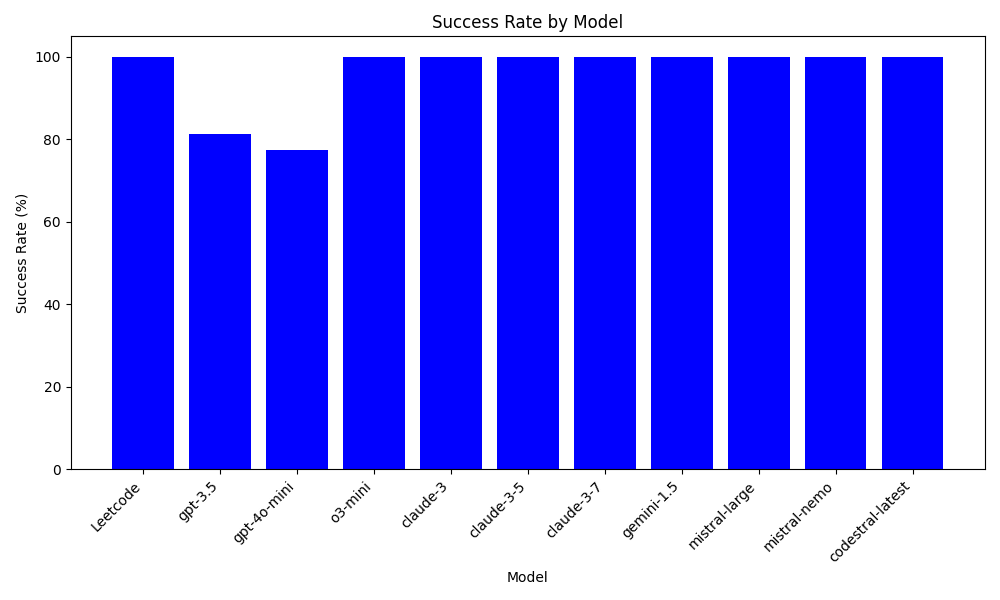
\includegraphics[width=15cm]{attachments/Success_Rate.png}
    \caption{Success Rate by Model} 
\end{figure}



\subsubsection{Runtime Performance}

As shown in Figure 2, LeetCode solutions exhibited the fastest runtime performance, indicating their computational efficiency. In contrast, GPT-4 exhibited slightly slower performance than GPT-3.5, potentially due to its more complex problem-solving mechanisms. Claude and Gemini demonstrated moderate runtime, emphasizing their balanced optimization between speed and accuracy.

\begin{figure}[H]
    \centering
    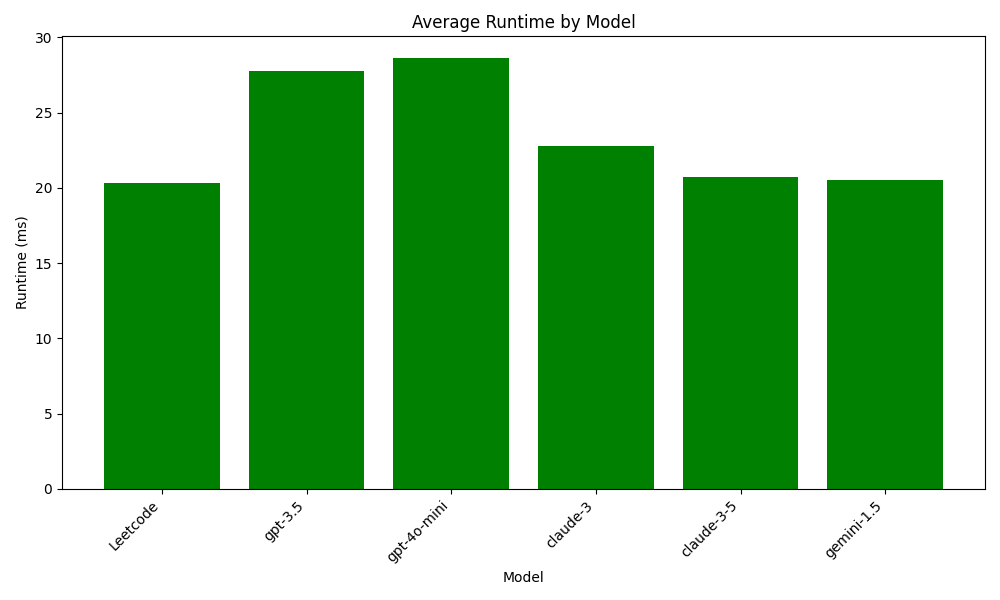
\includegraphics[width=15cm]{attachments/Average_Runtime.png}
    \caption{Average Runtime by Model} 
\end{figure}

\subsubsection{Memory Usage}

Figure 3 highlights the average memory consumption of each model. GPT-3.5 and GPT-4 had the highest memory usage, reflecting their reliance on extensive context processing. Claude and Gemini consumed less memory, showing their efficiency in managing resource utilization. LeetCode solutions required the least memory, indicating their lightweight implementations.

\begin{figure}[H]
    \centering
    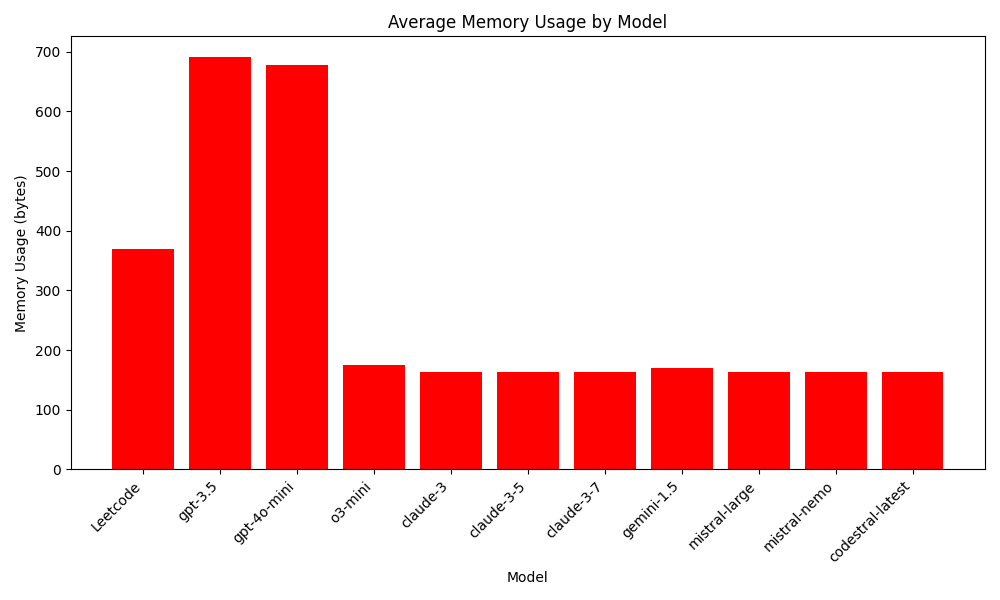
\includegraphics[width=15cm]{attachments/Average_Memory_Usage.png}
    \caption{Average Memory Usage by Model} 
\end{figure}

\subsection{Comparative Performance}

The comparative analysis revealed the trade-offs between speed, accuracy, and memory efficiency across the models. LeetCode solutions set a robust baseline with high accuracy and optimal resource utilization. GPT-3.5 and GPT-4 stood out for their advanced code generation capabilities but required higher computational resources. Claude and Gemini provided competitive performance with slightly lower resource demands, making them suitable for scenarios where memory efficiency is critical.



\subsection{Patterns and Insights}


Several patterns emerged from the analysis. First, the AI models demonstrated consistent success rates across easy and medium problems but showed variability on harder problems, particularly when edge cases or complex logic were involved. This indicates that while AI models excel at standard tasks, they may struggle with unconventional scenarios that require deeper reasoning or specialized knowledge.

Second, runtime and memory usage varied significantly between models. Models like GPT-4, which prioritize contextual understanding, tend to use more memory and exhibit slower runtimes compared to leaner models like Claude. These differences suggest that model selection should align with specific task requirements, balancing efficiency and accuracy.

Overall, the results underscore the growing potential of AI in programming while highlighting areas for improvement. The insights gained from this benchmark provide a foundation for refining AI systems and optimizing their application in real-world software engineering contexts.


















% \section{Implications and Future Directions}

% How AI models can augment current software engineering workflows (e.g., code generation, debugging, and testing).

% Potential changes to roles in the industry (e.g., humans focusing on higher-level tasks while AI handles routine coding).

% Use of AI in education or recruitment (e.g., automated assessment of programming skills).

% \subsection{Implications of Findings for Software Engineering}

% \subsubsection{Selection and Categorization of Programming Problems}

% Impact of problem diversity on AI performance.

% Lessons learned about problem selection and its role in meaningful AI evaluation.

% Recommendations for creating better problem sets in future research.

% \subsubsection{Characteristics of the Problem Set}

% How problem complexity affects AI performance.

% Importance of testing AI models on problems that mirror real-world software engineering challenges.

% The characteristics of the problem set play a crucial role in evaluating the true capabilities of AI models, as the complexity and nature of problems directly influence their performance. The problems used in this study were carefully curated to cover a wide range of scenarios that reflect both theoretical concepts and practical applications in software engineering.

% Problem complexity significantly affects AI performance. Simpler problems, often categorized as "easy," typically involve straightforward logic or basic algorithmic steps, such as iterating through an array or performing simple mathematical calculations. These problems serve as a baseline to assess the AI's ability to produce syntactically and logically correct solutions. AI models generally perform well on these tasks, as they require minimal contextual understanding and rely on commonly observed programming patterns.

% In contrast, more complex problems introduce layers of difficulty that challenge the AI's ability to reason, interpret, and optimize. Medium-difficulty problems often require intermediate skills such as recursion, efficient use of data structures like trees or heaps, or solving problems with moderate constraints. Hard problems push these boundaries further by demanding advanced algorithmic solutions, deep contextual understanding, and the ability to manage multiple interdependent variables. These challenges expose limitations in AI models, such as struggles with abstraction, lack of creativity in designing novel solutions, and inefficiency when faced with computationally intensive tasks.

% The inclusion of problems that mirror real-world software engineering scenarios is crucial for meaningful evaluation. Real-world challenges often involve incomplete or ambiguous problem statements, require multi-step reasoning, or necessitate balancing competing priorities like performance and readability. By incorporating such problems, the study ensures that the evaluation goes beyond textbook scenarios to assess the AI's practical utility. For example, problems that require handling edge cases, implementing scalable solutions, or integrating with existing systems offer valuable insights into the model’s readiness for deployment in professional environments.

% This diverse and thoughtfully constructed problem set enables a comprehensive understanding of the strengths and weaknesses of AI models. It highlights not only their technical capabilities but also their potential limitations when faced with real-world complexity, ultimately guiding future research and development in AI-driven programming tools.
% \subsection{Challenges and Limitations}

% Limitations of the study (e.g., focus on Leetcode, which may not reflect real-world scenarios).

% Challenges in evaluating non-deterministic AI outputs.

% Biases in the dataset or prompts that may influence AI performance.

% \subsection{Future Potential}

% The evolution of AI in software engineering presents a range of opportunities for advancing its role beyond current capabilities. As these models grow more sophisticated, they may achieve a deeper understanding of problem contexts, allowing them to address challenges involving ambiguity or incomplete information with greater precision. By refining their ability to interpret complex requirements, AI systems could become indispensable for tackling tasks that demand both technical knowledge and contextual reasoning.

% In addition to independent problem-solving, AI has the potential to become a more effective collaborator in team-based programming environments. By integrating seamlessly into workflows, these models could assist developers in real time, suggesting optimizations, identifying errors, and improving overall code quality. Such advancements would position AI as a trusted partner in the development process, augmenting rather than replacing human expertise.

% Another promising direction lies in enabling AI to handle large-scale, real-world projects. While current models are adept at solving isolated problems, future systems could extend their functionality to manage multi-file software projects with complex dependencies. This would open doors to applications in fields such as enterprise software development, where AI could assist in creating, maintaining, and scaling systems efficiently.

% The expansion of benchmarks and evaluation frameworks will also play a critical role in shaping the trajectory of AI in programming. By introducing benchmarks that better reflect real-world challenges, such as collaborative tasks or system design problems, researchers can encourage the development of models that align closely with industry needs. This will help bridge the gap between academic research and practical applications, ensuring AI evolves in ways that are directly beneficial to software engineering.

% The ethical implications of relying on AI for critical systems also demand attention. As these systems become more capable, it will be essential to address concerns such as accountability, transparency, and the potential displacement of human roles. By prioritizing responsible development and deployment, AI can be integrated into software engineering in a way that maximizes its benefits while minimizing risks.

% Future advancements in AI for software engineering are likely to reshape the profession in profound ways, enhancing productivity, enabling new possibilities, and driving innovation across the field. As these systems continue to evolve, their role will become increasingly central to the way software is designed, developed, and maintained.








% Suggestions for improving AI models (e.g., better training on real-world coding patterns, handling ambiguities).

% Expanding evaluations to include team-based programming or larger-scale projects.

% Creation of additional benchmarks to assess AI performance in different software engineering tasks (Use my old ideas).



% Do not add the code in Appendix, it is not necessary.